% =====================================================================
% ejercicio08.tex
% Responsabilidad única: barrer distintos valores de k sobre los datos
% estandarizados y analizar el trade-off entre Accuracy, Recall y F1.
% =====================================================================
\subsection{Ejercicio 8 --- Efecto del número de vecinos $k$}

\begin{table}[H]
\centering
\begin{tabular}{rrrrr}
\toprule
$k$ & Accuracy & Precision & Recall & F1 \\
\midrule
1  & 0.9044 & 0.2496 & 0.2144 & \textbf{0.2307} \\
3  & 0.9276 & 0.3978 & 0.1621 & 0.2303 \\
5  & 0.9329 & 0.4936 & 0.1357 & 0.2128 \\
7  & 0.9345 & 0.5412 & 0.1277 & 0.2066 \\
9  & \textbf{0.9350} & 0.5652 & 0.1167 & 0.1935 \\
11 & 0.9346 & 0.5583 & 0.1027 & 0.1735 \\
15 & 0.9343 & 0.5549 & 0.0883 & 0.1523 \\
21 & 0.9348 & 0.5863 & 0.0813 & 0.1428 \\
\bottomrule
\end{tabular}
\caption{Métricas por valor de $k$ (datos estandarizados).}
\end{table}

\begin{figure}[H]
    \centering
    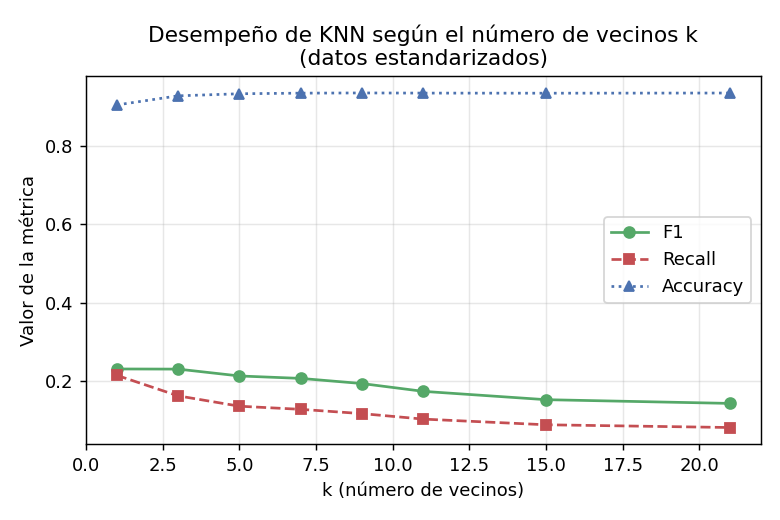
\includegraphics[width=0.7\textwidth]{figuras/ex8_k_vs_metricas.png}
    \caption{Desempeño de KNN según el número de vecinos $k$.}
\end{figure}

\begin{enumerate}

\item \textbf{Mejor F1:} $k=1$ ($F1=0.2307$).

\item \textbf{Mejor Recall:} $k=1$ ($\text{Recall}=0.2144$).

\item \textbf{Mejor Accuracy:} $k=9$ ($\text{Accuracy}=0.9350$).

\item \textbf{¿Coinciden los tres criterios en el mismo modelo?}
No, pues F1 y Recall se maximizan en $k=1$ mientras que Accuracy se
maximiza en $k=9$, y esto tiene una razón de fondo: Al aumentar $k$ el
modelo promedia sobre vecindarios cada vez más grandes que, dado el
fuerte desbalance de clases ($93\%/7\%$), terminan dominados por
vecinos de la clase mayoritaria, empujando las predicciones hacia la
clase 0 y sacrificando Recall a cambio de un Accuracy apenas mayor,
mientras que $k=1$, al fijarse solo en el vecino más próximo, es mucho
más sensible a los pocos vecinos positivos cercanos, favoreciendo el
Recall aunque a costa de una mayor varianza (más falsos positivos,
como en el Ejercicio 10).

\end{enumerate}
